\subsection{Phòng chơi}
Sau khi đã vào 1 phòng chơi bất kỳ, nhân vật của người chơi sẽ xuất hiện trong bản đồ.
\begin{figure}[H]
    \centering
    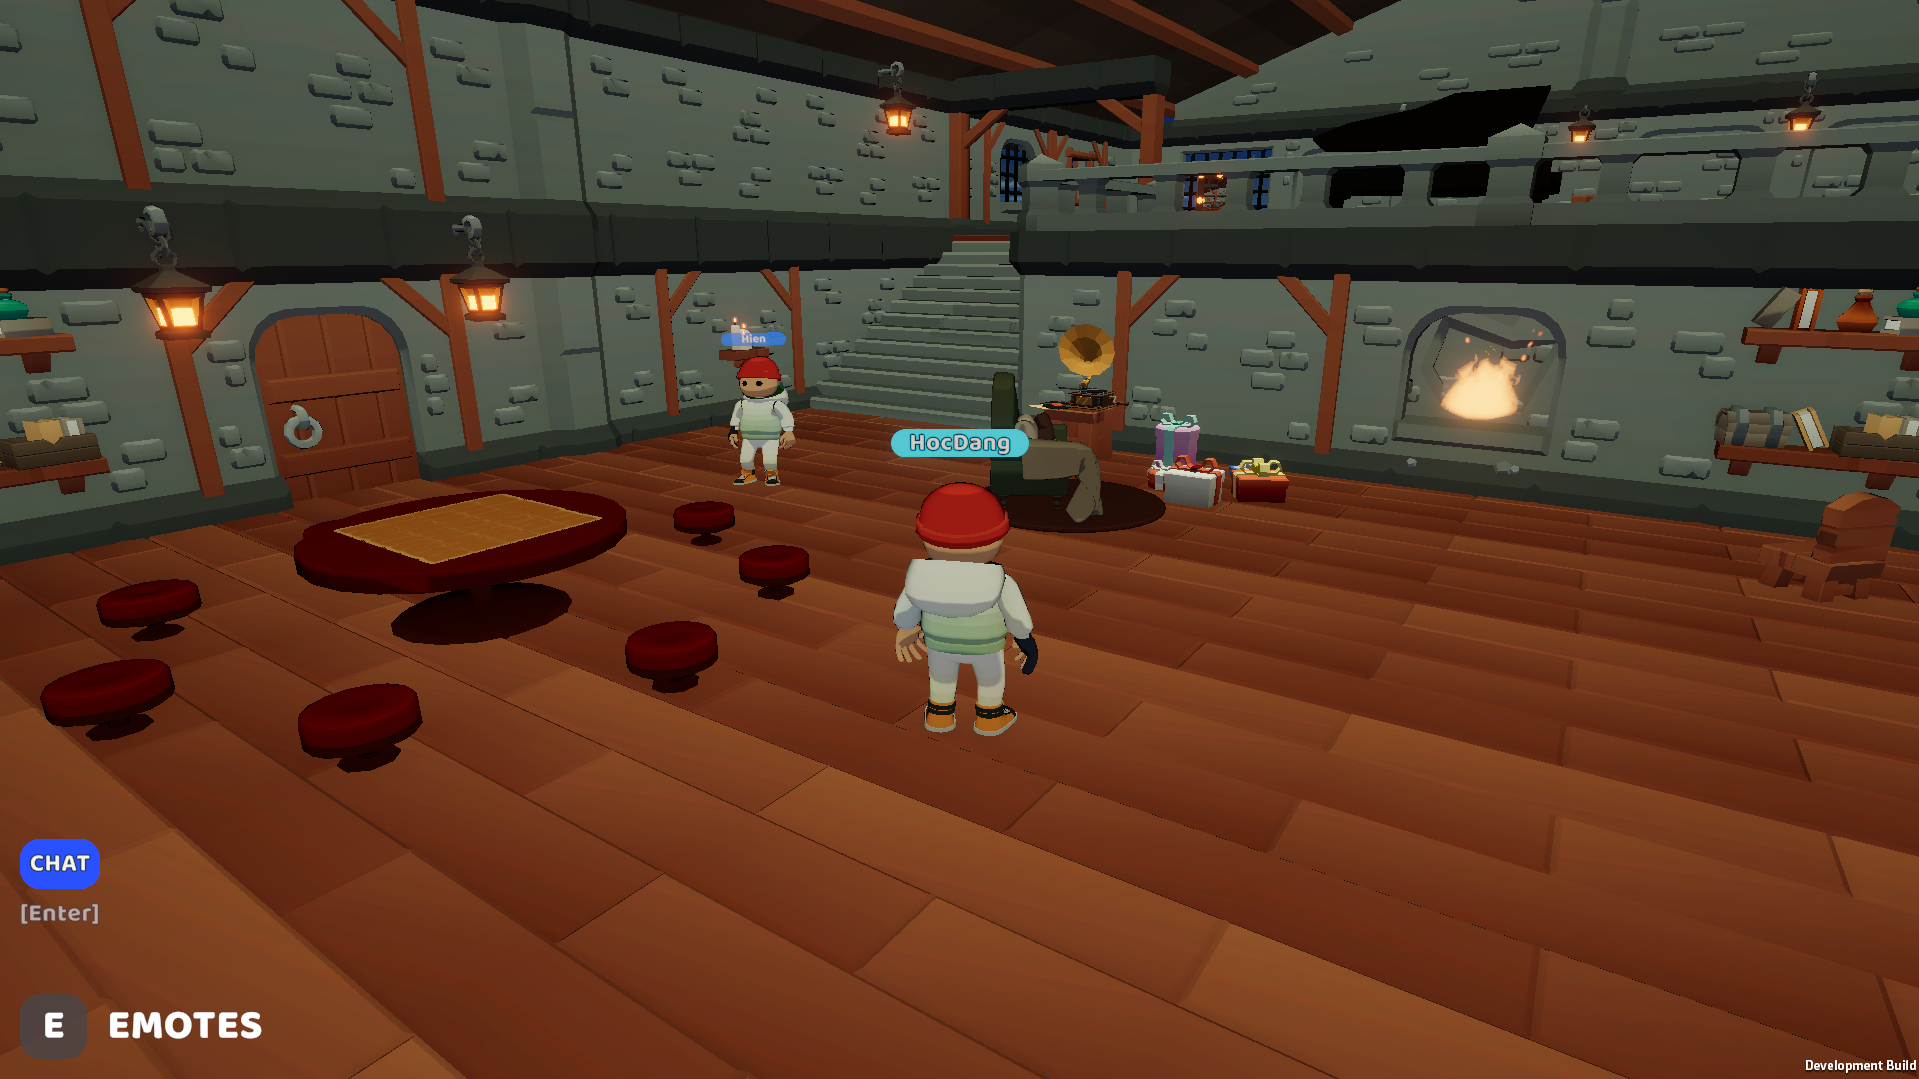
\includegraphics[width=0.75\linewidth]{10.Kết quả/images/DugeonMap.png}
    \caption{Screenshot màn hình bản đồ Dungeon Cabin của trò chơi}
    \label{fig:placeholder}
\end{figure}

\begin{figure}[H]
    \centering
    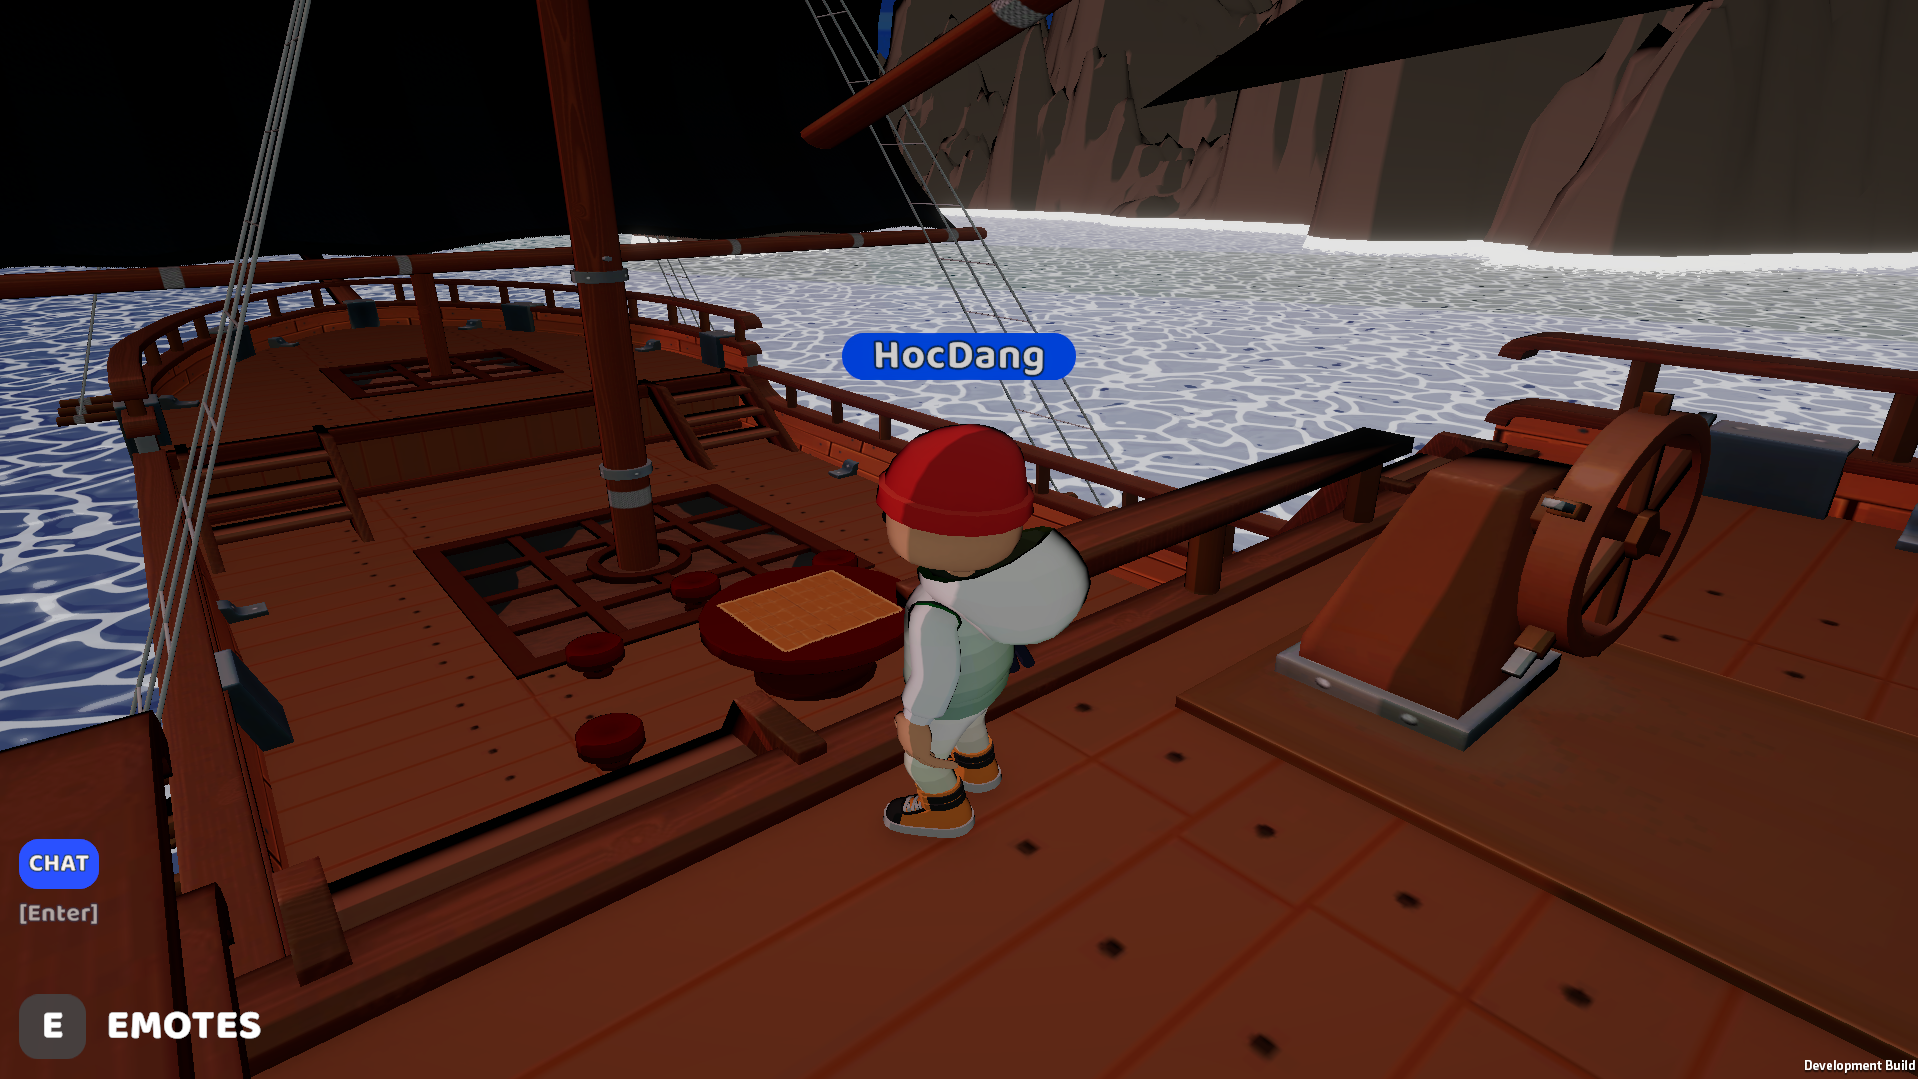
\includegraphics[width=0.75\linewidth]{10.Kết quả/images/BattleShipMap.png}
    \caption{Screenshot màn hình bản đồ Battle Ship của trò chơi}
    \label{fig:placeholder}
\end{figure}

Sau khi xuất hiện trong bản đồ, người chơi có thể đến gần các chiếc ghế xung quanh chiếc bàn và nhấn giữ nút "F" để ngồi vào bàn, khi đó sẽ hiện ra giao diện cấu hình cho game mode gồm 2 mdoe là classic (Saboteur gốc) và Day Night (Saboteur kết hợp với Ma sói).
\begin{figure}[H]
    \centering
    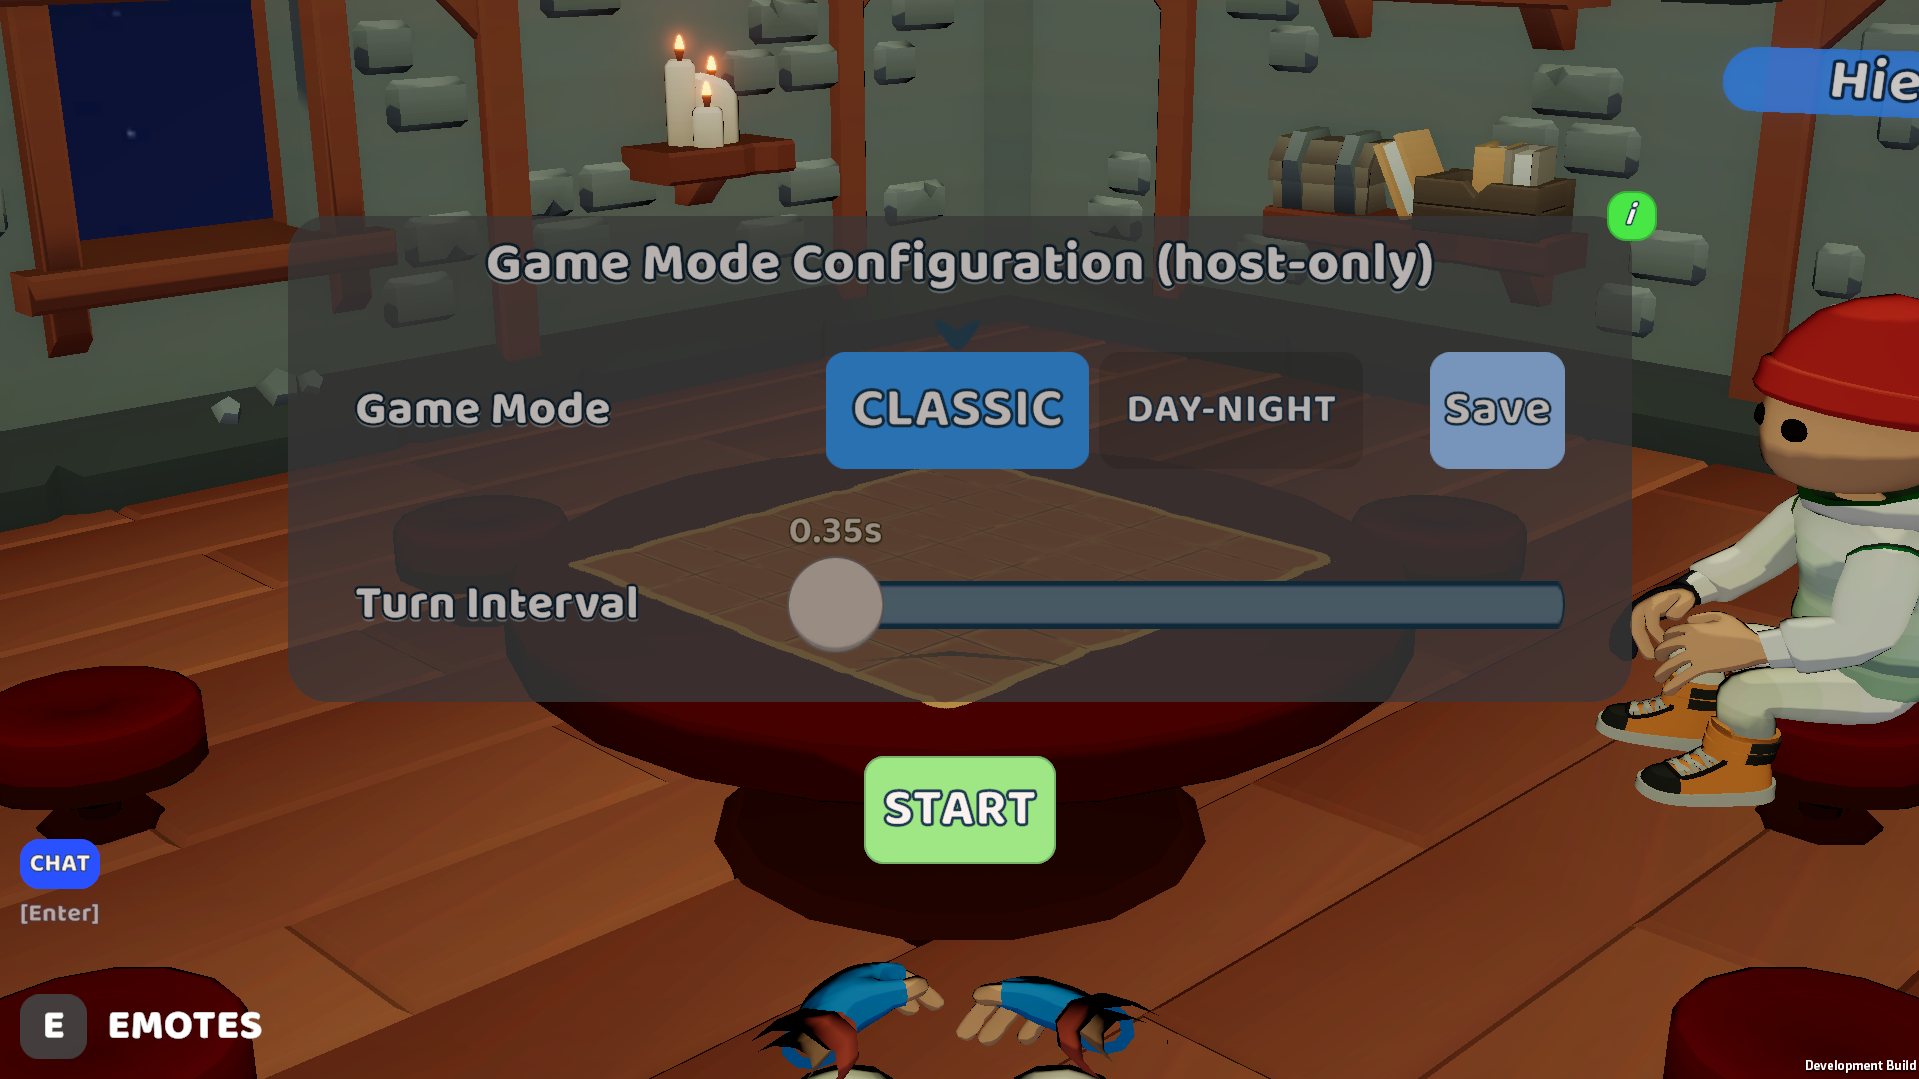
\includegraphics[width=0.75\linewidth]{10.Kết quả/images/ClassicConfig.png}
    \caption{Screenshot màn hình cấu hình Classic mode của trò chơi}
    \label{fig:placeholder}
\end{figure}

\begin{figure}[H]
    \centering
    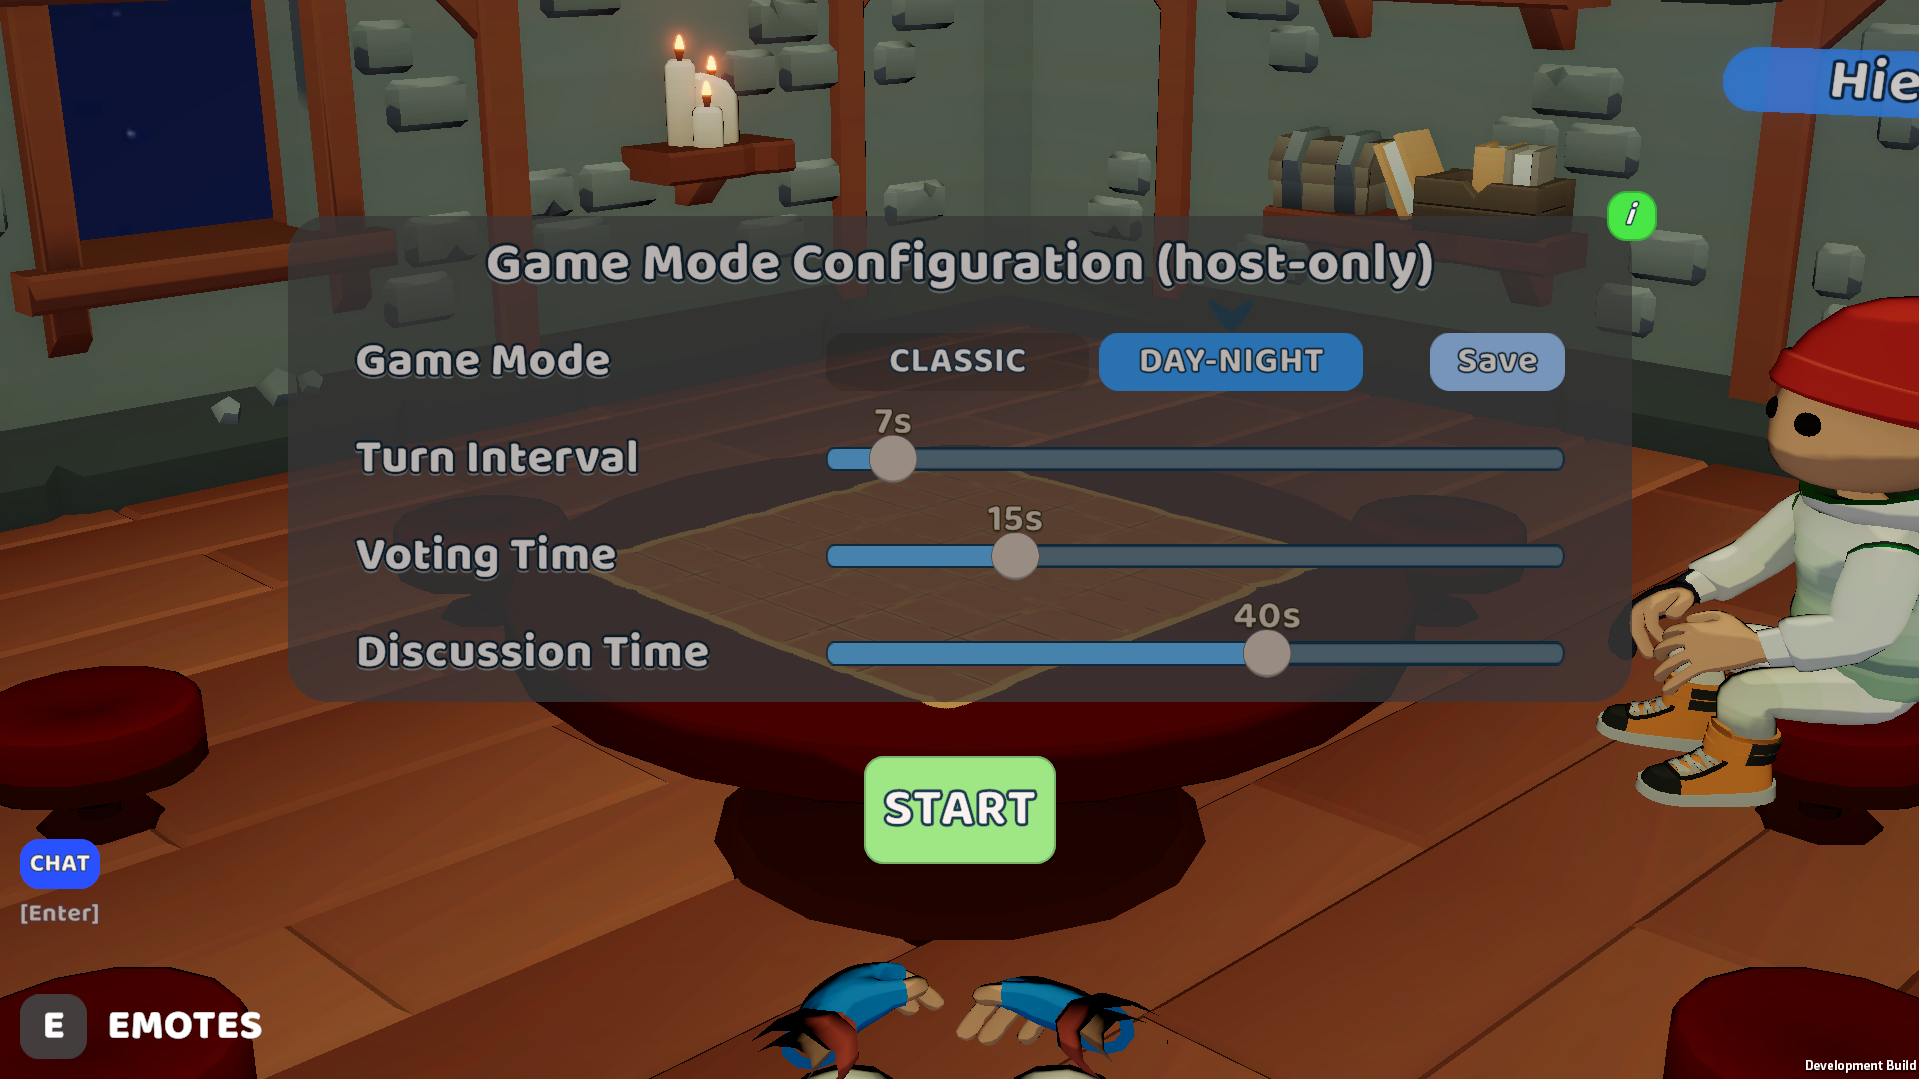
\includegraphics[width=0.75\linewidth]{10.Kết quả/images/DayNightConfig.png}
    \caption{Screenshot màn hình cấu hình Day Night mode của trò chơi}
    \label{fig:placeholder}
\end{figure}
Sau khi điều chỉnh thông số xong, người chơi chỉ cần nhấn nút "Save" và Start để bắt đầu vào trò chơi (chỉ chủ phòng mới có thể điều chỉnh thông số được).
\\
\begin{itemize}
    \item Classic Mode
        Tại đây, người chơi có thể chơi theo kim đồng hồ như Saboteur gốc.
        \begin{figure} [H]
            \centering
            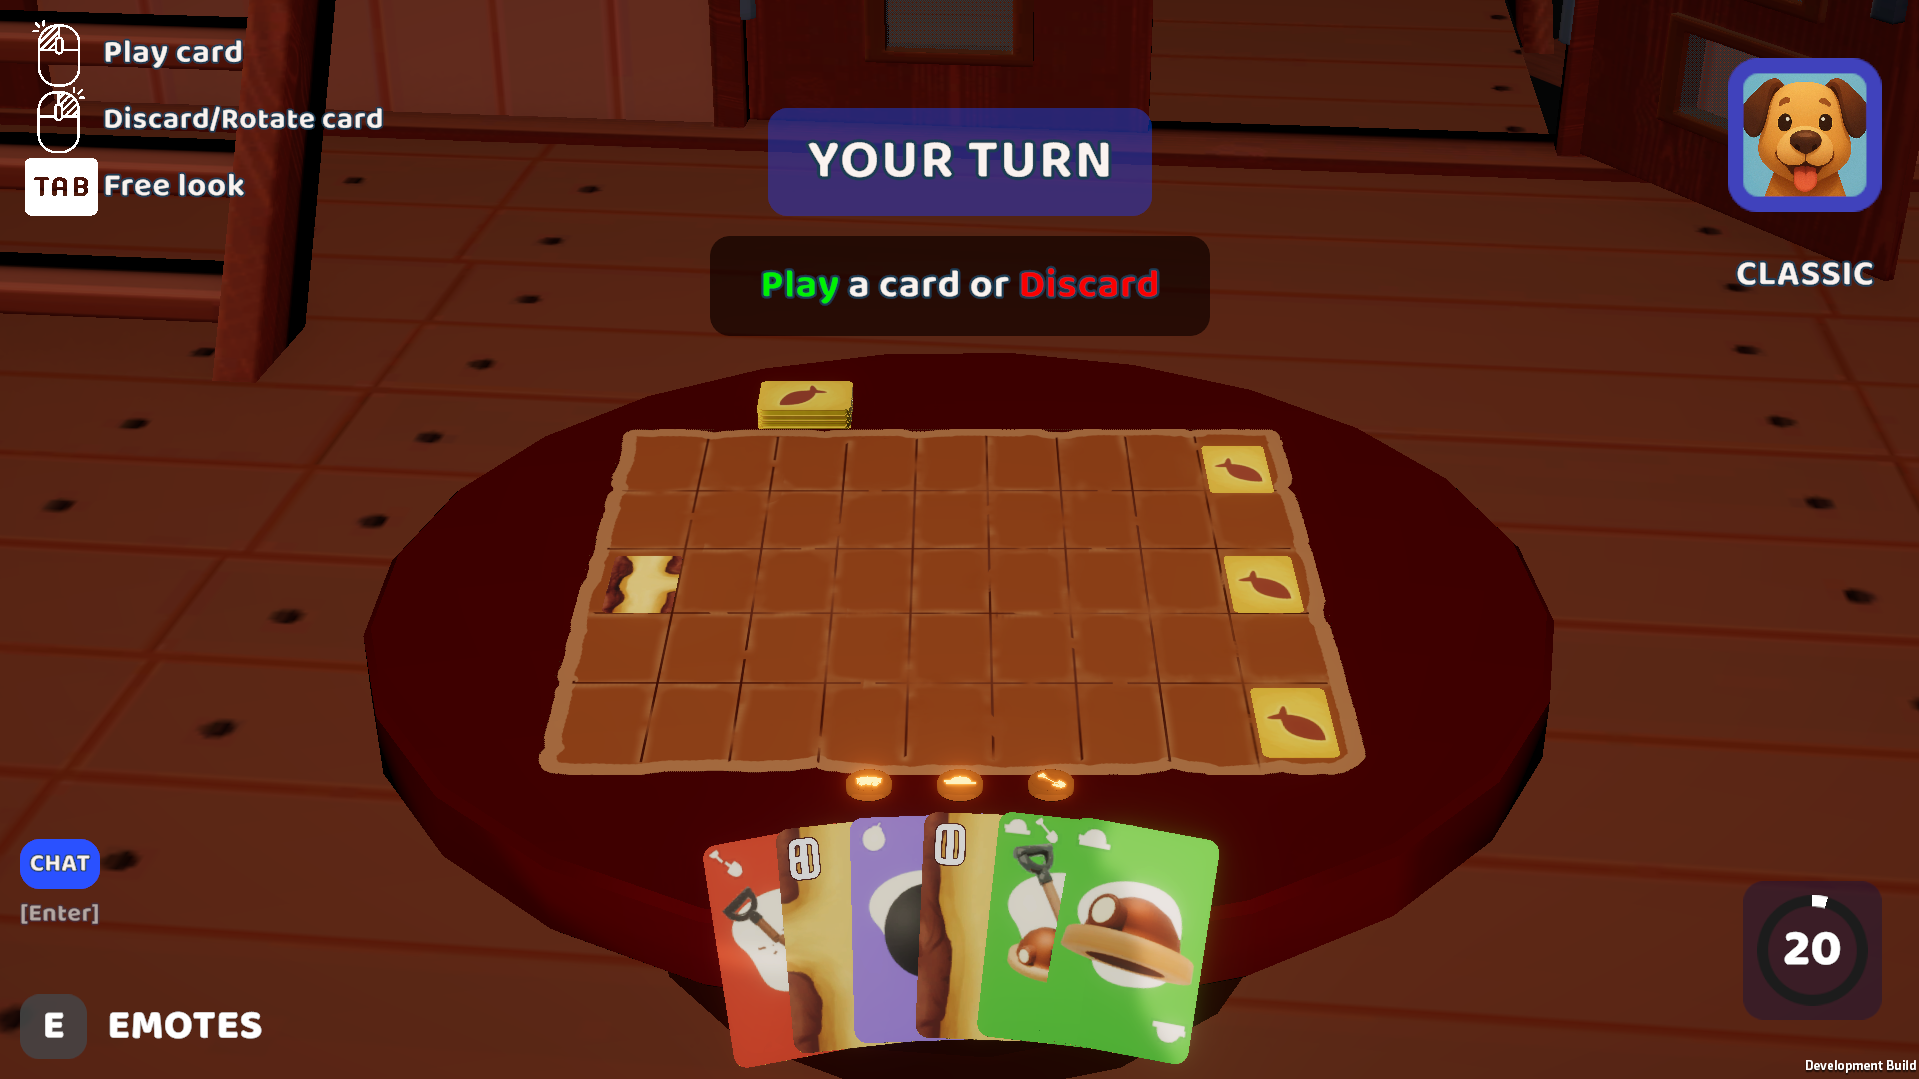
\includegraphics[width=0.75\linewidth]{10.Kết quả//images/ClassicMode.png}
            \caption{Screenshot màn hình bắt đầu Classic Mode của trò chơi}
            \label{fig:placeholder}
        \end{figure}
        Ở day phase, người chơi có thể thực hiện các hành động tự do như đặt đường, phá rối người khác, sử dụng các thẻ chức năng mà không sợ bị người khác thấy (trừ những người đã sử dụng thẻ nhìn xuyên đêm). Sau khi thực hiện 1 hành động xong thì sẽ kết thúc lượt.
    \item Day Night Mode
        \begin{figure} [H]
            \centering
            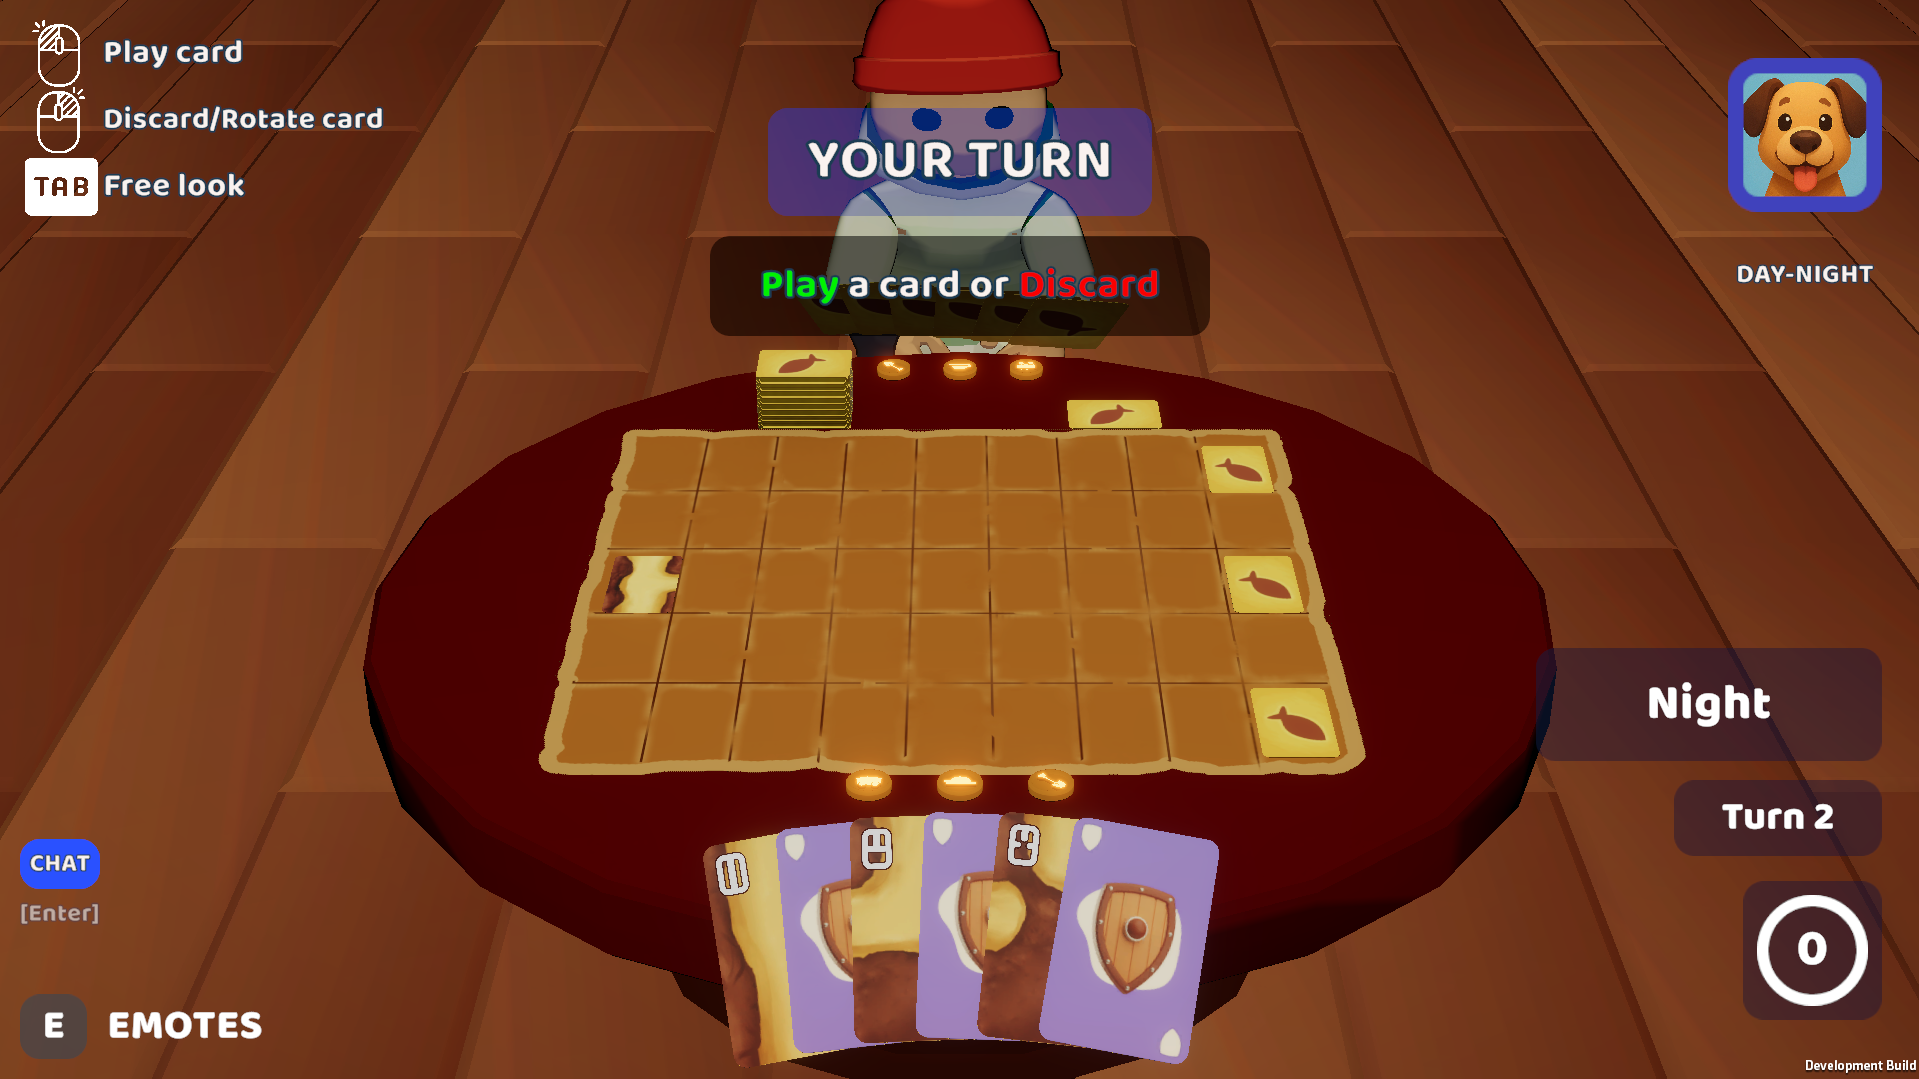
\includegraphics[width=0.75\linewidth]{10.Kết quả//images/DayPhase.png}
            \caption{Screenshot màn hình bắt đầu Day phase trong Day Night Mode của trò chơi}
            \label{fig:placeholder}
        \end{figure}
        Ở night phase, người chơi sẽ không thể nhìn được đang đến lượt ai hay ai đang làm gì, trừ khi đã sử dụng thẻ nhìn xuyên đêm. Chỉ khi sang phase mới như discussion hoặc đến lượt của bản thân gì mới có thể thấy được hiện trạng của board.
        \begin{figure} [H]
            \centering
            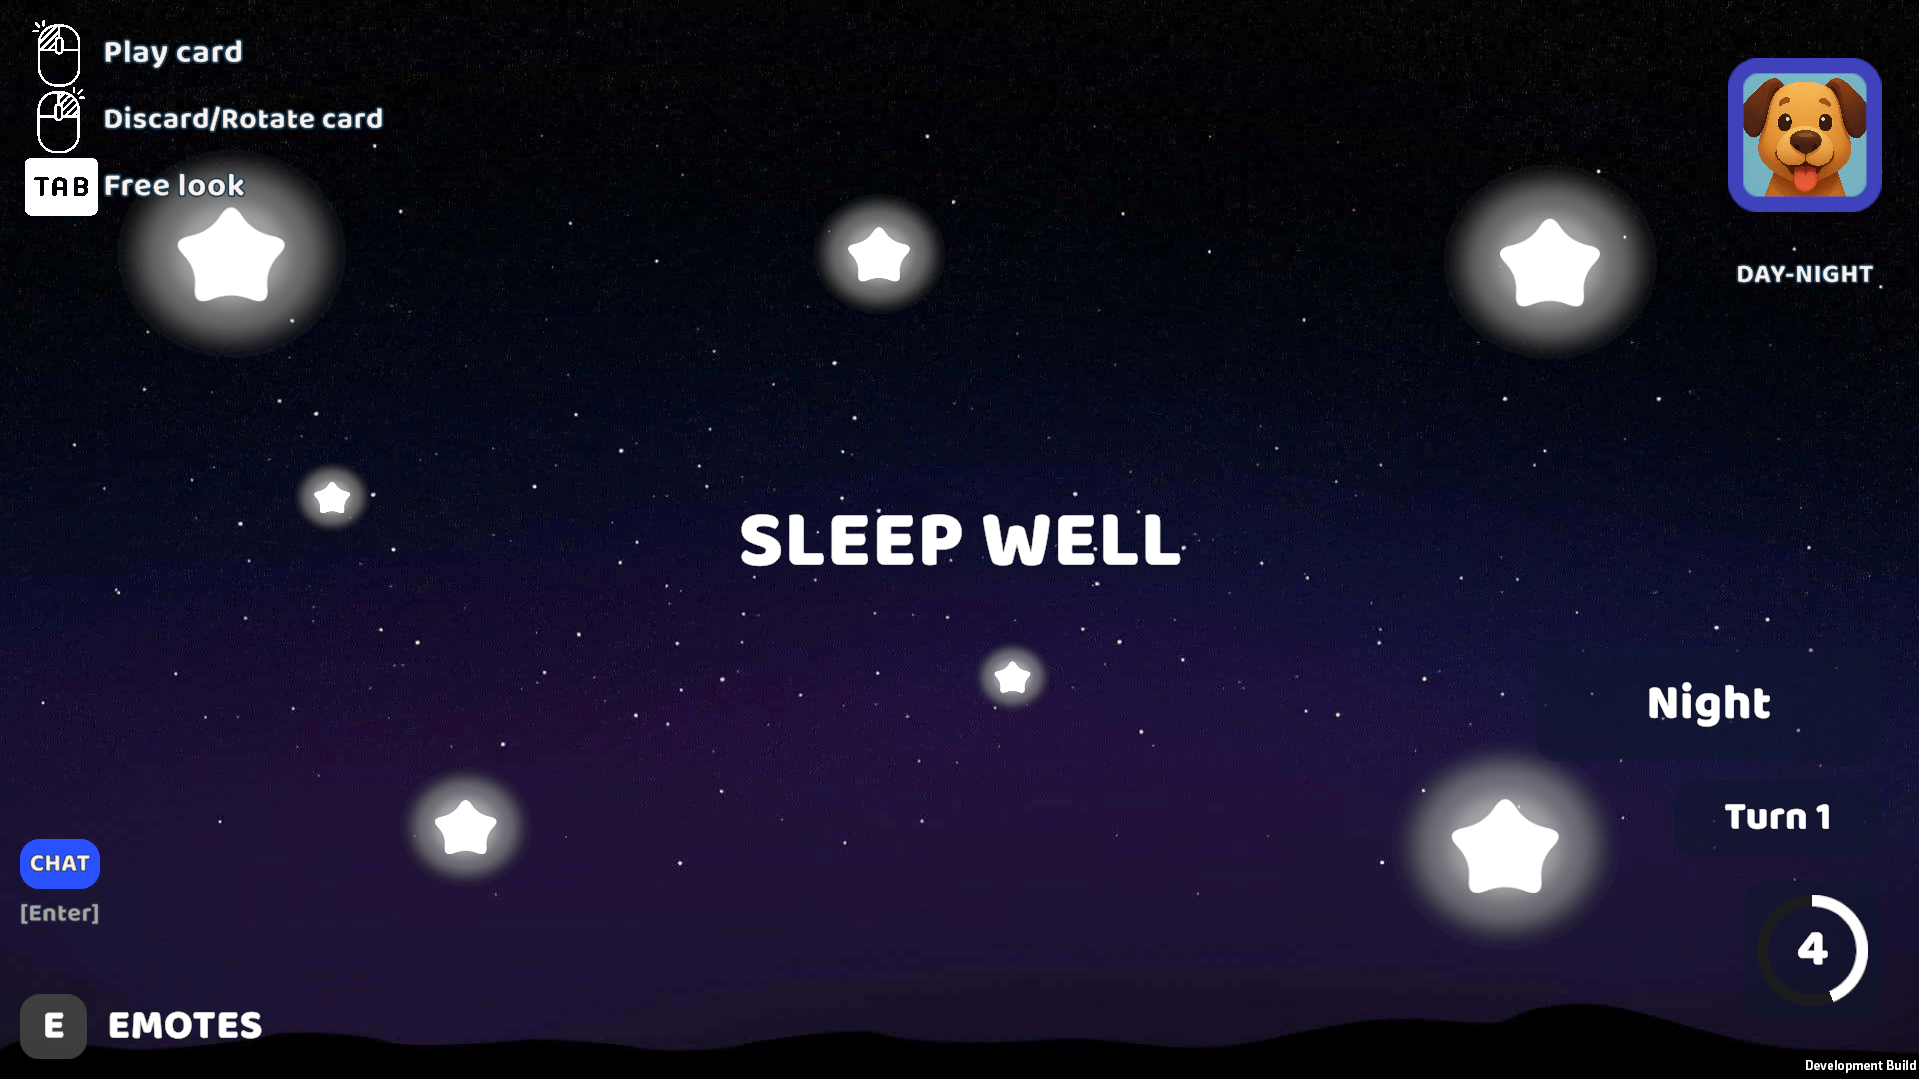
\includegraphics[width=0.75\linewidth]{10.Kết quả//images/NightPhase.png}
            \caption{Screenshot màn hình bắt đầu Night phase trong Day Night Mode của trò chơi}
            \label{fig:placeholder}
        \end{figure}
        Ở discussion phase, các người chơi có thể thấy được hiện trạng của board và thảo luận xem ai đã phá rối hay có vấn đề gì để có thể tiếp tục voting phase.
        
        \begin{figure} [H]
            \centering
            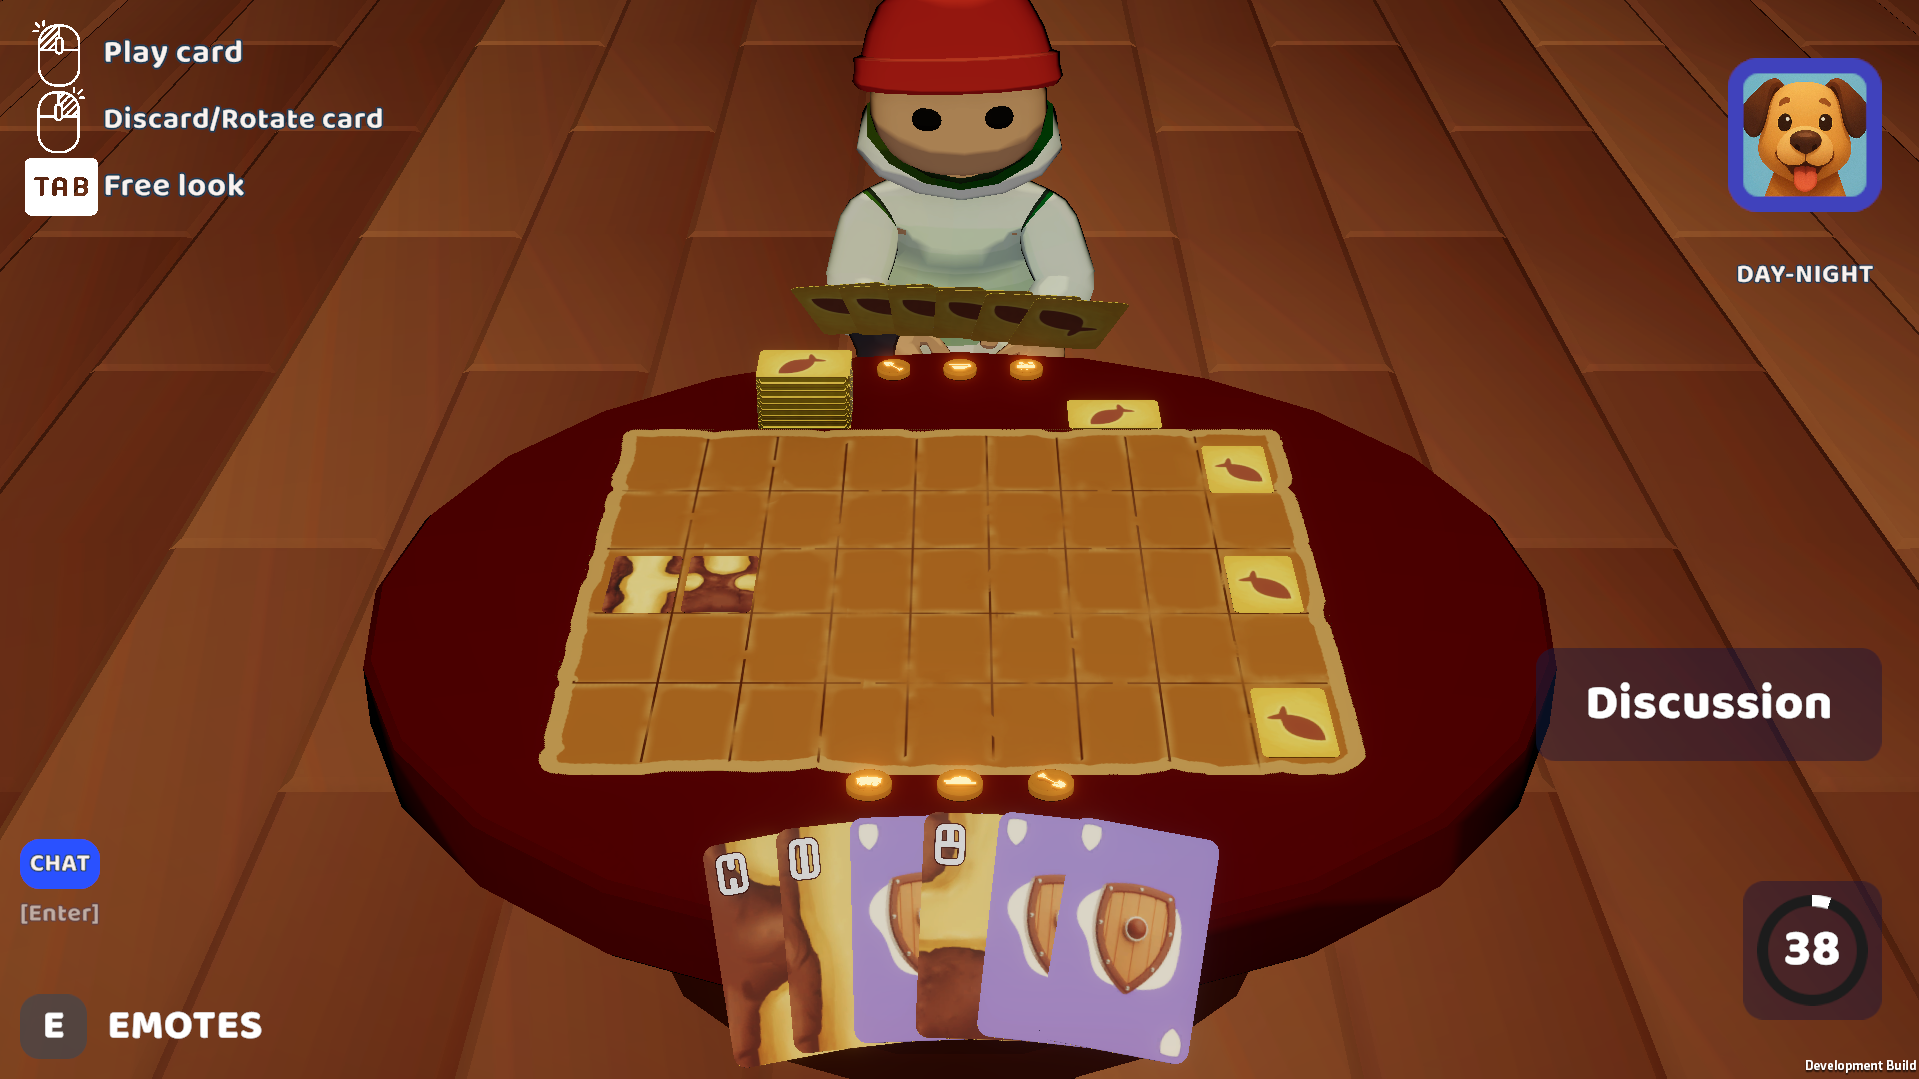
\includegraphics[width=0.75\linewidth]{10.Kết quả//images/DiscussionPhase.png}
            \caption{Screenshot màn hình bắt đầu Discussion phase trong Day Night Mode của trò chơi}
            \label{fig:placeholder}
        \end{figure}
        Ở voting phase, các người chơi có thể bầu chọn những ai mà mình nghi ngờ nhằm mục đích cấm 1 lượt chơi của người đó ở đêm kế tiếp.
        \begin{figure} [H]
            \centering
            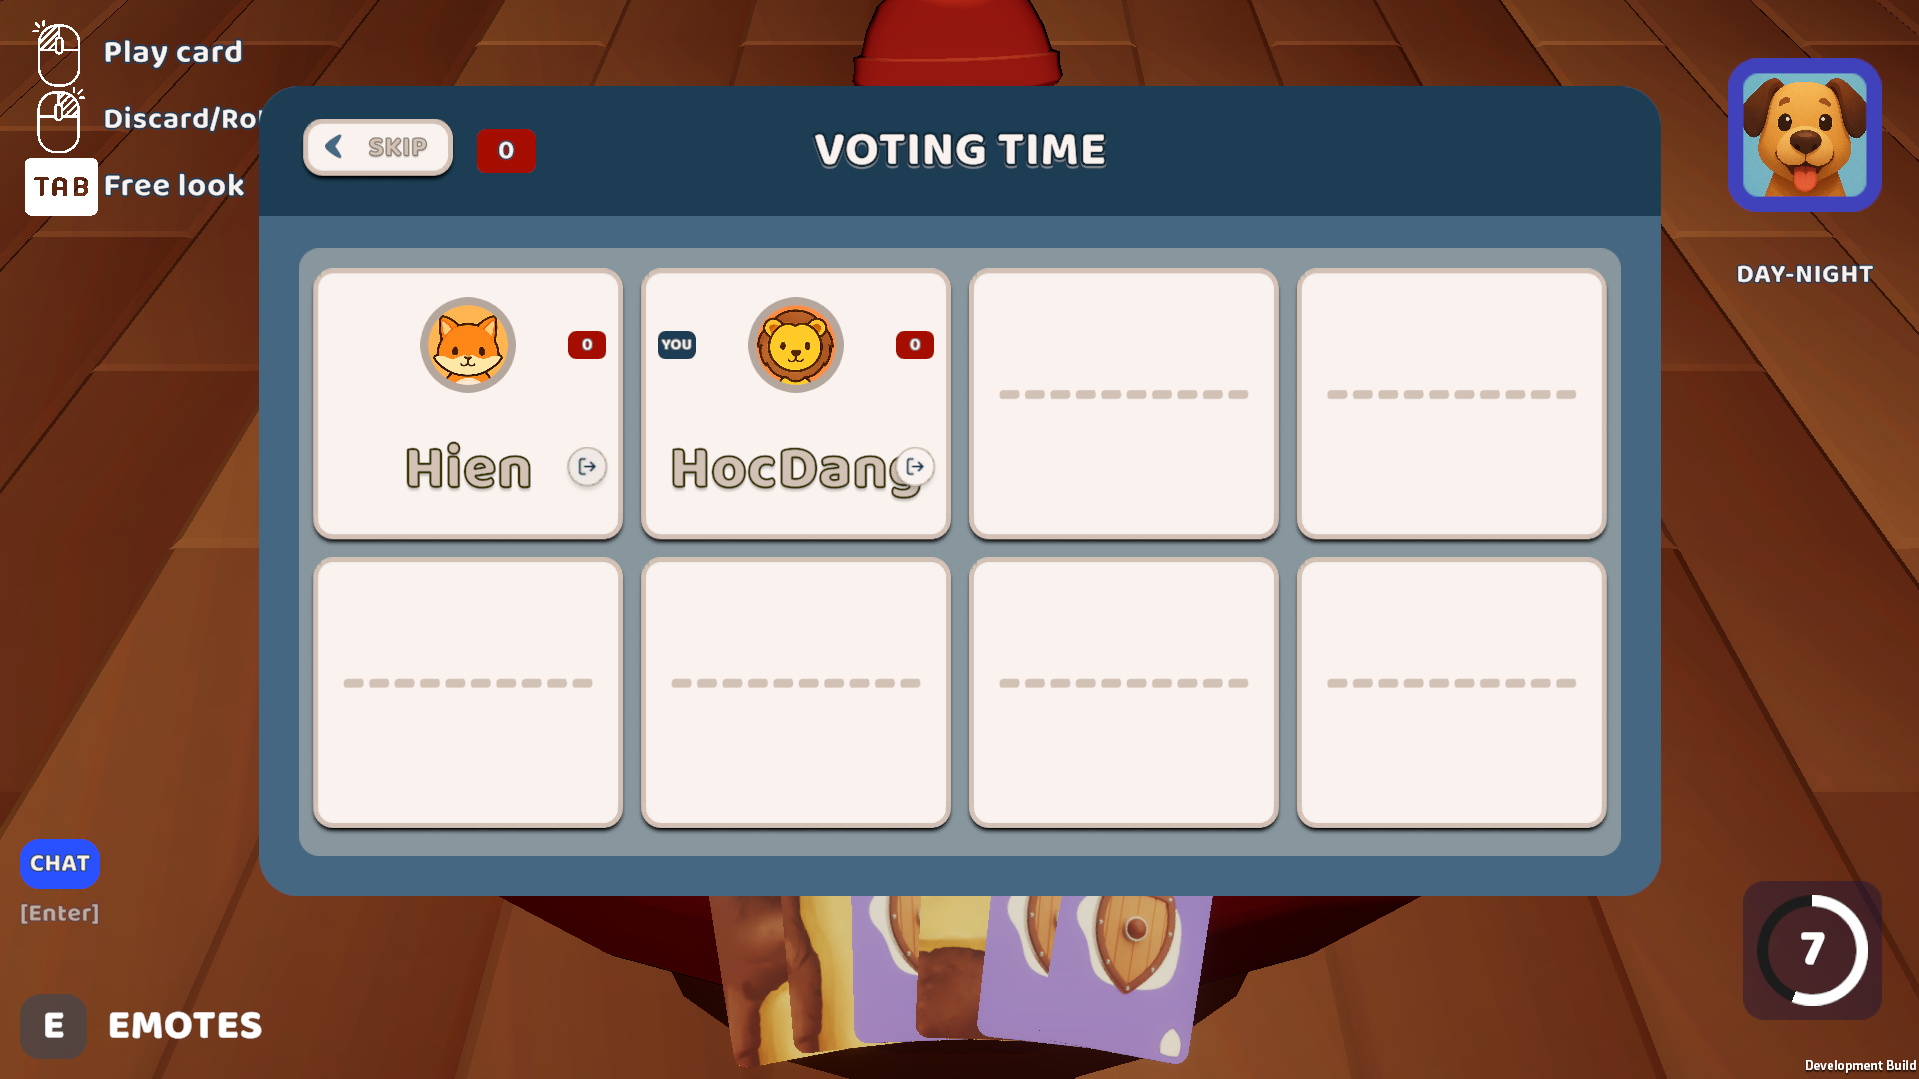
\includegraphics[width=0.75\linewidth]{10.Kết quả//images/VotingPhase.png}
            \caption{Screenshot màn hình bắt đầu Voting phase trong Day Night Mode của trò chơi}
            \label{fig:placeholder}
        \end{figure}
\end{itemize}

\subsubsection{Menu}
Người chơi có thể mở giao diện Menu bằng cách nhấn nút "Esc" để có thể xem thông tin phòng chơi, thông tin trò chơi, ...
\begin{figure}[H]
    \centering
    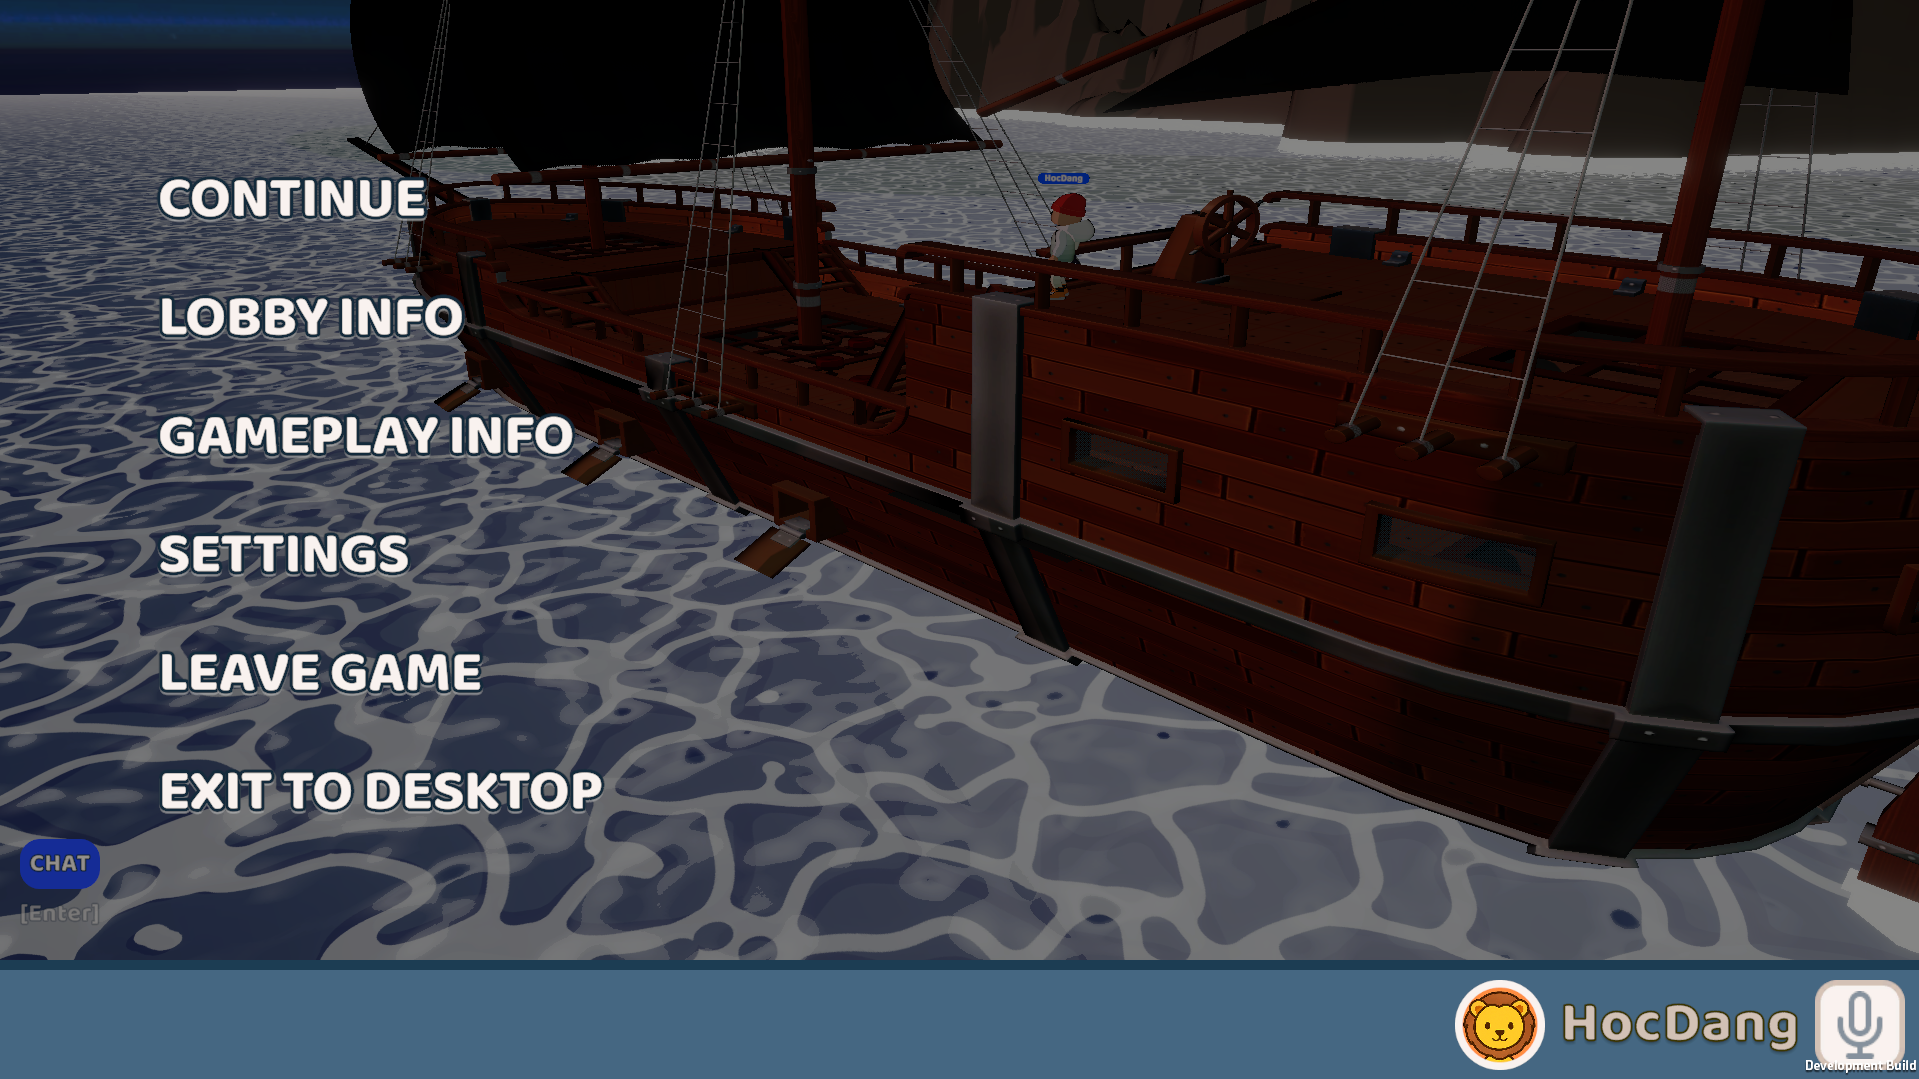
\includegraphics[width=0.75\linewidth]{10.Kết quả/images/MenuLobby.png}
    \caption{Screenshot màn hình Menu Lobby của trò chơi}
    \label{fig:placeholder}
\end{figure}
Người chơi có thể nhấn vào Lobby Info để xem thông tin phòng chơi như: có những ai, kết thúc game (nếu đang chơi board game), ... hoặc cũng có thể kick một người chơi ra khỏi phòng (chỉ chủ phòng mới làm được).
\begin{figure}[H]
    \centering
    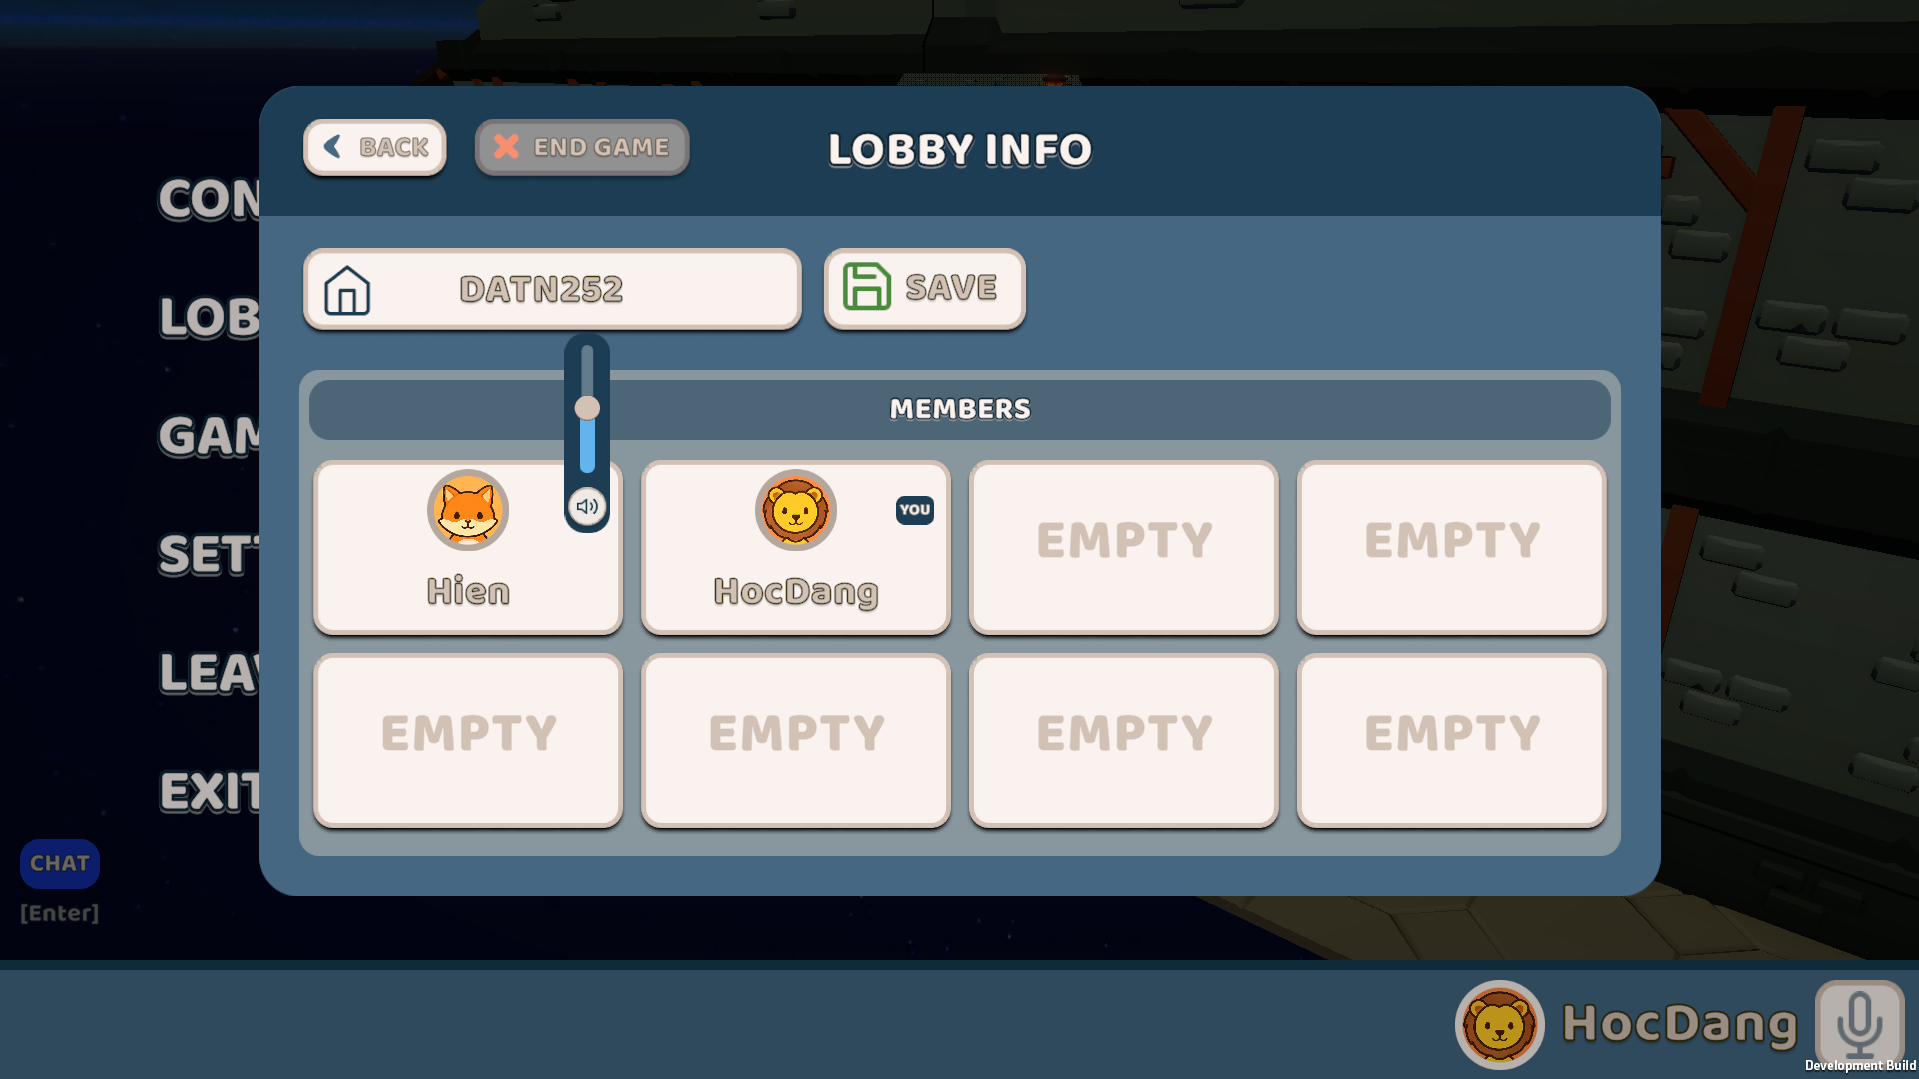
\includegraphics[width=0.75\linewidth]{10.Kết quả/images/LobbyInfo.png}
    \caption{Screenshot màn hình Lobby Info của trò chơi}
    \label{fig:placeholder}
\end{figure}
Người chơi cũng có thể nhấn vào Gameplay Info để xem luật chơi, các chức năng của các lá bài, ...
\begin{figure}[H]
    \centering
    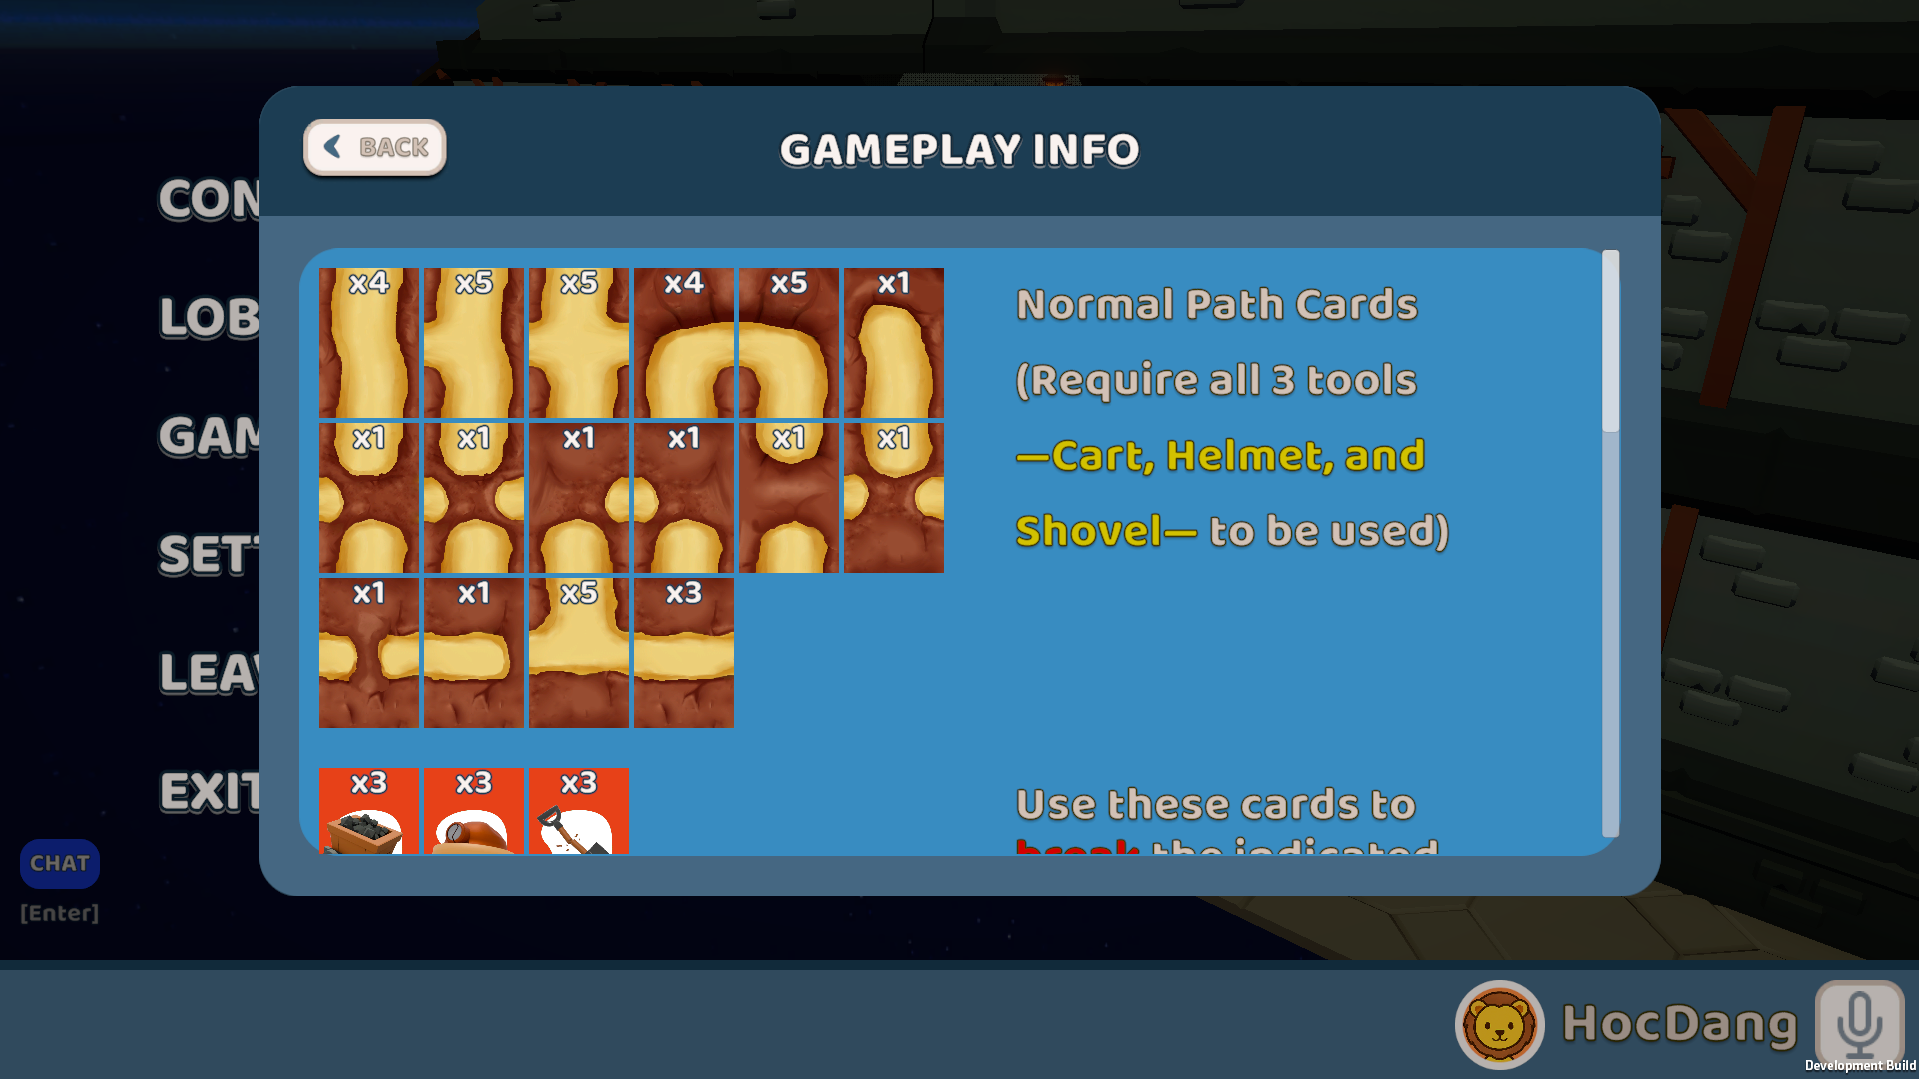
\includegraphics[width=0.75\linewidth]{10.Kết quả/images/PlayGameInfo.png}
    \caption{Screenshot màn hình Gameplay Info của trò chơi}
    \label{fig:placeholder}
\end{figure}
